\subsubsection{Instruction Set} \label{subsec: instructions-set}

The ZKVM module uses different spaces between instructions and memory addresses.
It is because the ZKVM module has sufficient space for use,
and using a unified space can make the column for storing constraints smaller, reducing overhead.


\textbf{register} \label{subsubsec: zkvm-executor-register}

    Currently, there are two main models for designing the L0 layer of the ZKVM memory hierarchy in the industry, one is the register model and the other is the stack model.
For the stack model, state updates are implemented according to the first-in-last-out model of the stack.The constraints are relatively simple.
However, the disadvantage is that accessing the state is not user-friendly.
It is not possible to use one instruction to randomly access data at a specific address in the stack. \\
In contrast, the register model only requires one instruction to complete a randomly read operation, while the stack model requires multiple pop and push operations.
Alternatively, to improve efficiency, swap-like instructions are added in the MidenVM design to optimize randomly accessed data in the stack.
For the register model, any registers can be randomly accessed.
However, the disadvantage is that the constraint model requires copy constraints for the upper and lower instructions and more columns for register selectors.
The columns in the trace table are larger than the stack model. \\
    As designed in the last version of the whitepaper,OlaVM selects a register model.There are 9 general-purpose registers.
The symbol denotes as  :$\texttt{r}_0 - \texttt{r}_{8}$.
The $\texttt{r}_{8}$ is used as $\texttt{fp}$ (frame pointer). $\texttt{fp}$ is the alias of $\texttt{r}_{8}$.

The PC (program counter) pointer of a loaded program initially points to the instruction at address 0.
As instructions are executed, the value of the address pointed to by the PC changes.
If a jump or call instruction is not executed, the address stored in the PC register is incremented by 1 for each instruction executed, unless the instruction uses an immediate value, in which case the PC is incremented by 2.

The PSP (prophet stack pointer) register is used to alloc the prophet memory segment when ZkVM execute prophet code.In the initial state, set the prophet memory segment start address ($2^{64} - 2*2^{32}$) to this register.

\textbf{Olavm instructions}

To minimize the degree of constraints, The ZKVM model use reduced instruction set.

Olavm use Word (64bits) encode instruction.
An instruction is encoded with an opcode and up to three operands, which can be either a register or an immediate value.
An instruction encoding consists of the following 8 fields:
\begin{itemize}
    \item Field1: Field name: NULL.1 bit width,not used.
    \item Field2: Field name: OP1 immediate flag (OP1\_IMM, imm). 1-bit width. Set to 0, indicates that A is a register; set to 1, indicates that A is an immediate value.
    \item Field3: Field name: operation0 register (OP0\_REG, reg\_src1). 9-bit width. Indicates source op0 register index, index range from 0 to 8.
                  Set to 1 determine operating the register corresponding to the index, otherwise set to 0.
    \item Field4: Field name: operation1 register (OP1\_REG, reg\_src2). 9-bit width. Indicates source op1 register index, index range from 0 to 8.
                  Set to 1 determine operating the register corresponding to the index, otherwise set to 0.If all 9 bits set to 0, indicates use PSP (prophet stack pointer) register.
    \item Field5: Field name: destination register (DST\_REG, reg\_dst). 9-bit width. Indicates destination register index, index range from 0 to 8.
                  Set to 1 determine operating the register corresponding to the index, otherwise set to 0.
    \item Field6: Field name: opcode selector (opcode\_sel). 21-bit width. Indicates the opcode type, set to 1 determine executing the opcode, otherwise set to 0.
    \item Field7: Field name: padding bits (paddings). 14-bit width.
                  All bits padding by 0, will be used in the future.
    \item Field8: Field name: immediate data (immediate). This field is an option, determined by field2 if field2 is set to 1.
                  This field indicates an immediate value, This field is 2 Word wide.
\end{itemize}

The instruction set of the ZkVM model is as below, A denoted intermediate or register:
\begin{table}[!ht]
    \resizebox{\textwidth}{!}{%
        \begin{tabular}{|c|c|c|c|c|}
            \hline
            \textit{Type}  & \textit{Instruction} & \textit{Operands} & \textit{Description} & \textit{flag} \\ \hline
            \multirow{2}{*}{Field Operation}  & ADD & ri rj A & Compute rj + A and store the result in ri &   \\ \cline{2-5}
            & MUL & ri rj A & Compute rj * A and store the the result in ri &  \\ \cline{2-5}
            & NOT & ri A &  Compute not A and store the the result in ri &  \\  \hline
            \multirow{2}{*}{Cmp}  & EQ & ri rj A & Equality comparison and store the the result in ri & rj = A \\ \cline{2-5}
            & NEQ & ri rj A &  check whether rj is not equal A and store the the result in ri & rj != A \\ \cline{2-5}
            & ASSERT & ri  A & Assert ri == A and vm will hang up if assertion fail &  \\  \hline
            Move & MOV & ri A & Copy the data of A to ri &  \\ \hline
            \multirow{5}{*}{Flow} & JMP & A & Set pc equal A &  \\ \cline{2-5}
            & END &  & only appears at the end of the program &  \\  \cline{2-5}
            & CJMP & rj A & If rj = 1, set pc equal A, else increment pc as usual &  \\  \cline{2-5}
            & CALL & A & \multicolumn{1}{l|}{\begin{tabular}[c]{@{}l@{}}The Call instruction consists of the following steps\\ 1. store return pc to the frame address [fp-1].\\ 2. jump to the address A\end{tabular}} &  \\  \cline{2-5}
            & RET &  & \multicolumn{1}{l|}{\begin{tabular}[c]{@{}l@{}}The Ret instruction consists of the following two steps\\ 1. use the memory address stored in the fp register to find the returned pc and jump to the location of the returned pc.\\ 2. update the fp register to the fp before the call\end{tabular}} &  \\ \hline
            \multirow{2}{*}{RAM} & MLOAD & ri [A, imm] & \multicolumn{1}{l|}{\begin{tabular}[c]{@{}l@{}}Read the value from memory [A+imm] and store it into ri. \\ imm is optional, can not represent. \\ A can be a intermediate data or register value.\\ if A is a  register, can follow a immediate data.\end{tabular}}&  \\ \cline{2-5}
            & MSTORE & [A, imm] rj & \multicolumn{1}{l|}{\begin{tabular}[c]{@{}l@{}}Read the value from register rj and store it into memory [A+imm]. \\ imm is optional, can not represent. \\ A can be a intermediate data or register value. \\ if A is a  register, can follow a immediate data.\end{tabular}}&  \\ \hline
            \multirow{8}{*}{BUILTIN} & RANGE CHECK & rj & range check the value in rj  &  \\ \cline{2-5}
            & AND & ri rj A &  Compute rj and A and store the the result in ri &  \\ \cline{2-5}
            & OR & ri rj A &  Compute rj or A and store the the result in ri &  \\ \cline{2-5}
            & XOR & ri rj A &  Compute rj xor A and store the the result in ri &  \\ \cline{2-5}
            & GTE & ri rj A &  check whether rj is great than or equal to A and store the the result in ri &  rj >= A \\ \hline
        \end{tabular}%
    }
    \caption{Instruction set}
    \label{table:instruction-set}
\end{table}

As per the above definition: instruction encoding uses 2W width when there is no immediate value, and 4W width when there is an immediate value.
The alloc principle of operand: when register status changes, the register is set as DST\_REG operand.
when the register state does not change, the register is set as OP0\_REG operand and OP1\_REG operand.
If only use one register status not changes, use OP1\_REG operand.
The instruction encodes format as the table below:

\begin{table}[!ht]
    \centering \resizebox{\linewidth}{!}{
        \begin{tabular}{*{16}{|c}|}
            \hline
            NULL & \multicolumn{1}{|c|}{OP1\_IMM}  & OP0\_R8 & OP0\_R7 & OP0\_R6 & OP0\_R5 & OP0\_R4 & OP0\_R3 & OP0\_R2 & OP0\_R1 & OP0\_R0
            & OP1\_R8 & OP1\_R7 & OP1\_R6 & OP1\_R5 & OP1\_R4  \\ \hline
            OP1\_R3 & OP1\_R2 & OP1\_R1 & OP1\_R0 & DST\_R8 & DST\_R7 & DST\_R6 & DST\_R5 & DST\_R4 & DST\_R3 & DST\_R2 & DST\_R1 & DST\_R0
            & ADD & MUL & EQ  \\ \hline
            ASSERT & MOV  & JMP & CJMP & CALL & RET & MLOAD & MSTORE & END & RANGE\_CHECK & AND & OR & XOR & NOT & NEQ & GTE \\ \hline
            \multicolumn{16}{|c|}{padding} \\ \hline
            \multicolumn{16}{|c|}{immediate data 48-63 bits}  \\ \hline
            \multicolumn{16}{|c|}{immediate data 32-47 bits}  \\ \hline
            \multicolumn{16}{|c|}{immediate data 16-31 bits}  \\ \hline
            \multicolumn{16}{|c|}{immediate data 0-15 bits}  \\ \hline
            15 & 14 & 13 & 12 & 11 & 10 & 9 & 8 & 7 & 6 & 5 & 4 & 3 & 2 & 1 & 0 \\ \hline
        \end{tabular}}
    \caption{OlaVM instruction encode format}
    \label{table: processor_instruction_decode}
\end{table}

The pseudocode for the state transition of executing instructions is as follows:
\begin{lstlisting}[language={}]
new_op:
opcode = opcode_list[instuction[pc].opcode_sel]
imm = instuction[pc].imm
ri = reg_dst
rj = reg_src1

if imm == 1:
    next = pc + 2
    A = immediate
else
    next = pc + 1
    A = reg_src2
endif

switch opcode:
    ADD:
        ri = rj + A
        break
    MUL:
        ri = rj * A
        break
    EQ:
        if rj == A:
            ri = 1
        else
            ri = 0
        break
    MOV:
        ri = A
        break
    JMP:
        pc = A
        goto new_op
    CJMP:
        if rj == 1:
            pc = A
        goto new_op
    CALL:
        [fp-1] = next
        pc = A
        goto new_op
    RET:
        fp = [fp-2]
        pc = [fp-1]
        goto new_op
    MLOAD:
        ri = [A]
        break
    MSTORE:
        [A] = ri
        break
    ASSERT:
        if ri != A:
           panic("ASSERT failed")
    RANGE_CHECK:
        insert ri value to rangetable trace table
        break
    AND:
        ri = rj & A
        break
    OR:
        ri = rj | A
        break
    XOR:
        ri = rj xor A
        break
    NOT:
        ri = not
        break
    NEQ:
        ri = rj != A
        break
    GTE:
        ri = rj >= A
        break
pc = next
goto new_op
\end{lstlisting}


\textbf{procedure call standard}

stack space to function.When executing a ret instruction, the fp decrease and reclaim stack space allocated to the function.
After executing a call instruction,fp points to the callee function stack.The return pc address stored in:\texttt{[fp-1]}, the caller fp address stored in \texttt{[fp-2]}, the first three input parameters stored in $\texttt{r}_1 - \texttt{r}_{3}$.
From the fourth parameter, the parameters are stored in descending order: \texttt{[fp-3]}, \texttt{[fp-4]} $\cdots$.
The local variables are stored in the stack from \texttt{[fp]} in ascending order.The return value stored in $\texttt{r}_0$.

For example: function \texttt{foo(a: felt, b: felt, c: felt, d: felt, e: felt)}, input parameters: \texttt{a=0x1, b=0x2, c=0x3, d=0x4, e=0x5}.
\begin{lstlisting}[label={lst:function_call}]
func foo(a: felt, b: felt, c: felt, d: felt, e: felt)
    let sum = 0;
    sum = a+b;
    sum = sum * c;
    sum = sum + d + e
    return ;
\end{lstlisting}

The \texttt{fp, pc} and memory status when function call as below (yellow represent memory address, red represent instruction address,blue represent registers):
\begin{figure}[!htp]
    \centering
    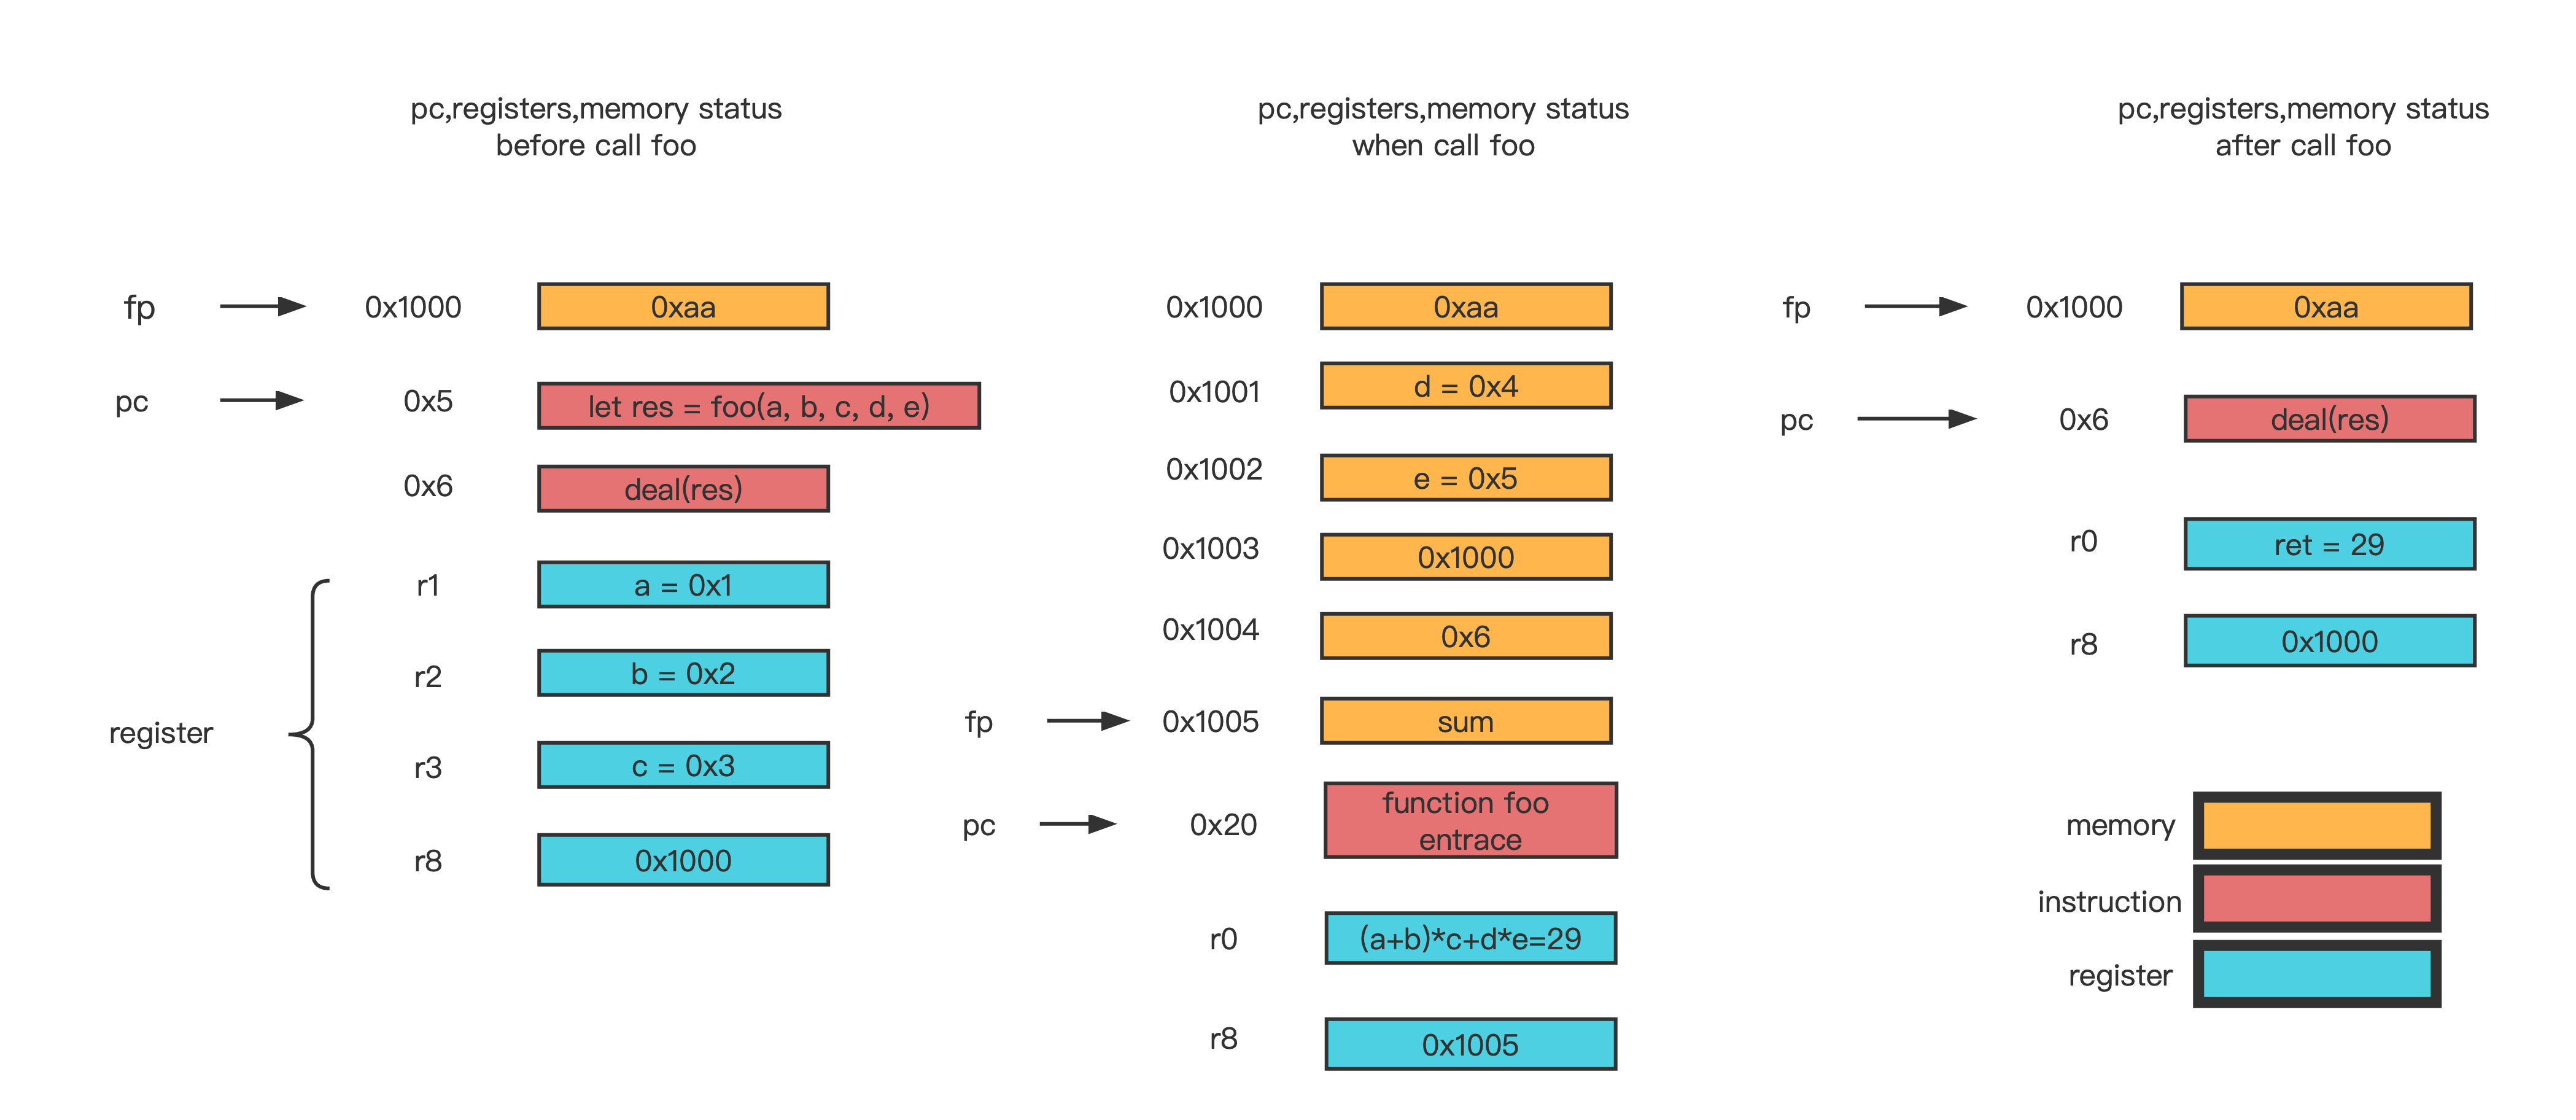
\includegraphics[width=1\textwidth]{olavm call.jpg}
    \caption{OlaVM function call model}
    \label{fig:processor call}
\end{figure}
